\documentclass{../../slides-style}

\slidetitle{Лекция 6: Структурные шаблоны}{14.03.2024}

\begin{document}

    \begin{frame}[plain]
        \titlepage
    \end{frame}

    \section{Введение}

    \begin{frame}
        \frametitle{Паттерны проектирования}
        \textbf{Шаблон проектирования} --- это повторимая архитектурная конструкция, являющаяся решением некоторой типичной технической проблемы
        \begin{itemize}
            \item Подходит для класса проблем
            \item Обеспечивает переиспользуемость знаний
            \item Позволяет унифицировать терминологию
            \item В удобной для изучения форме
            \item НЕ конкретный рецепт или указания к действию
        \end{itemize}
    \end{frame}

    \begin{frame}
        \frametitle{Паттерны и архитектурные стили}
        \begin{center}
            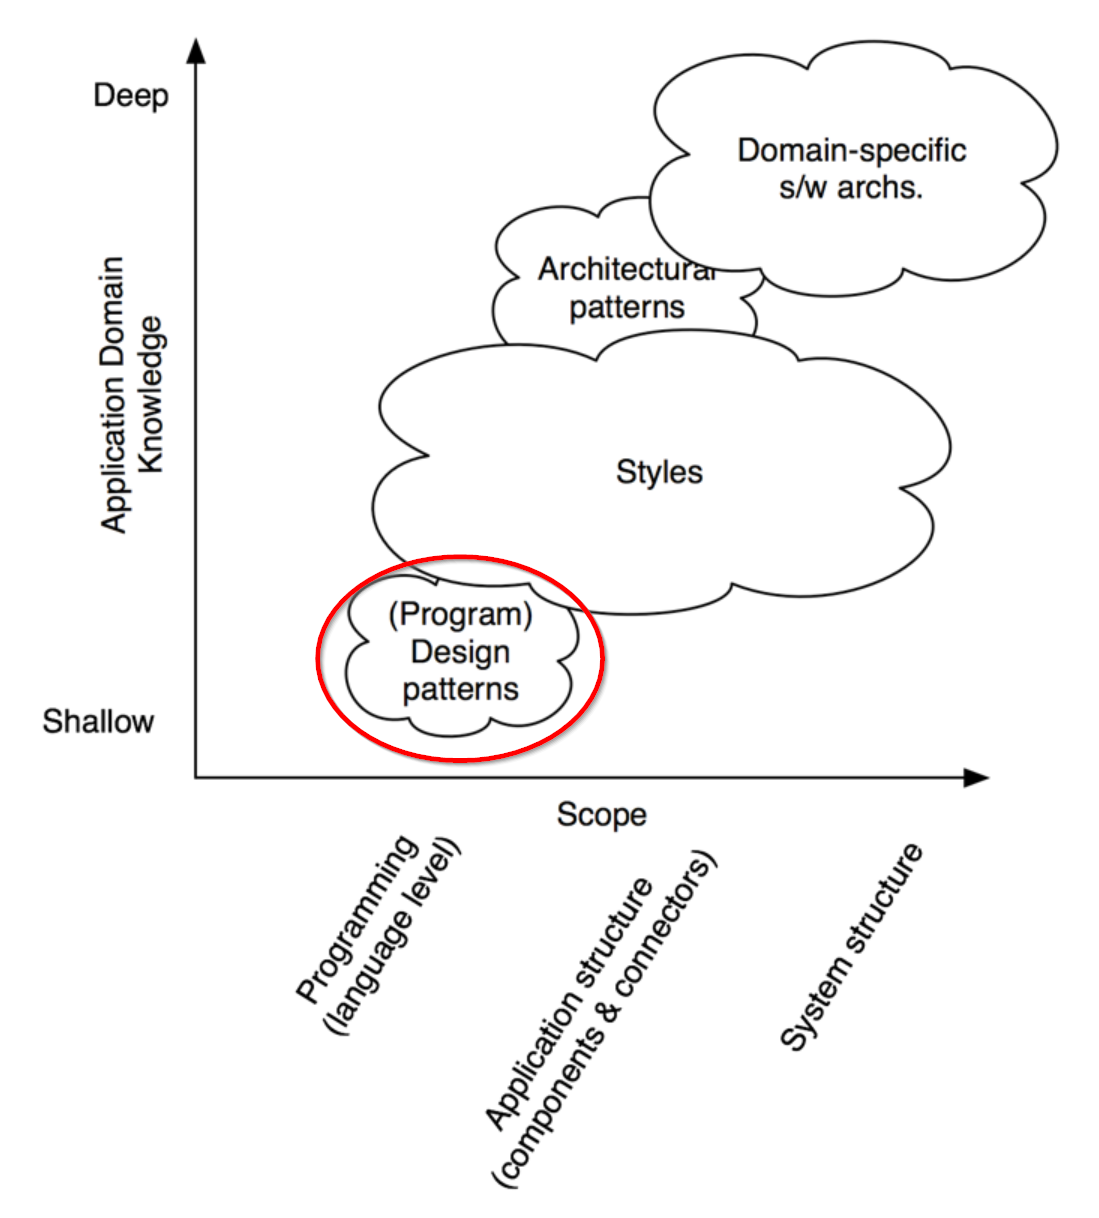
\includegraphics[width=0.5\textwidth]{architecturalStylesPatternsHighlighted.png}
            \attribution{N. Medvidovic}
        \end{center}
    \end{frame}

    \begin{frame}
        \frametitle{Книжка про паттерны}
        \framesubtitle{Must read!}

        \begin{columns}
            \begin{column}{0.6\textwidth}
                Приемы объектно-ориентированного проектирования. Паттерны проектирования

                Э. Гамма, Р. Хелм, Р. Джонсон, Дж. Влиссидес

                Design Patterns: Elements of Reusable Object-Oriented Software
            \end{column}
            \begin{column}{0.4\textwidth}
                \begin{center}
                    
\includegraphics[width=0.8\textwidth]{patternBookCover.png}
                \end{center}
            \end{column}
        \end{columns}
    \end{frame}

    \begin{frame}
        \frametitle{Начнём с примера}
        \framesubtitle{Текстовый редактор}
        WYSIWYG-редактор, основные вопросы:
        \begin{itemize}
            \item Структура документа
            \item Форматирование
            \item Создание привлекательного интерфейса пользователя
            \item Поддержка стандартов внешнего облика программы
            \item Операции пользователя, undo/redo
            \item Проверка правописания и расстановка переносов
        \end{itemize}
    \end{frame}

    \section{Паттерн ``Компоновщик''}

    \begin{frame}
        \frametitle{Структура документа}
        \begin{itemize}
            \item Документ --- множество графических элементов
            \begin{itemize}
                \item Организация в физическую структуру
                \item Средства UI для манипулирования структурой
            \end{itemize}
            \item Требования к внутреннему представлению
            \begin{itemize}
                \item Отслеживание внутренней структуры документа
                \item Генерирование визуального представления
                \item Отображение позиций экрана на внутреннее представление
            \end{itemize}
            \item Ограничения
            \begin{itemize}
                \item Текст и графика едины
                \item Простой и составной элементы едины
            \end{itemize}
        \end{itemize}
    \end{frame}

    \begin{frame}
        \frametitle{Рекурсивная композиция}
        \begin{center}
            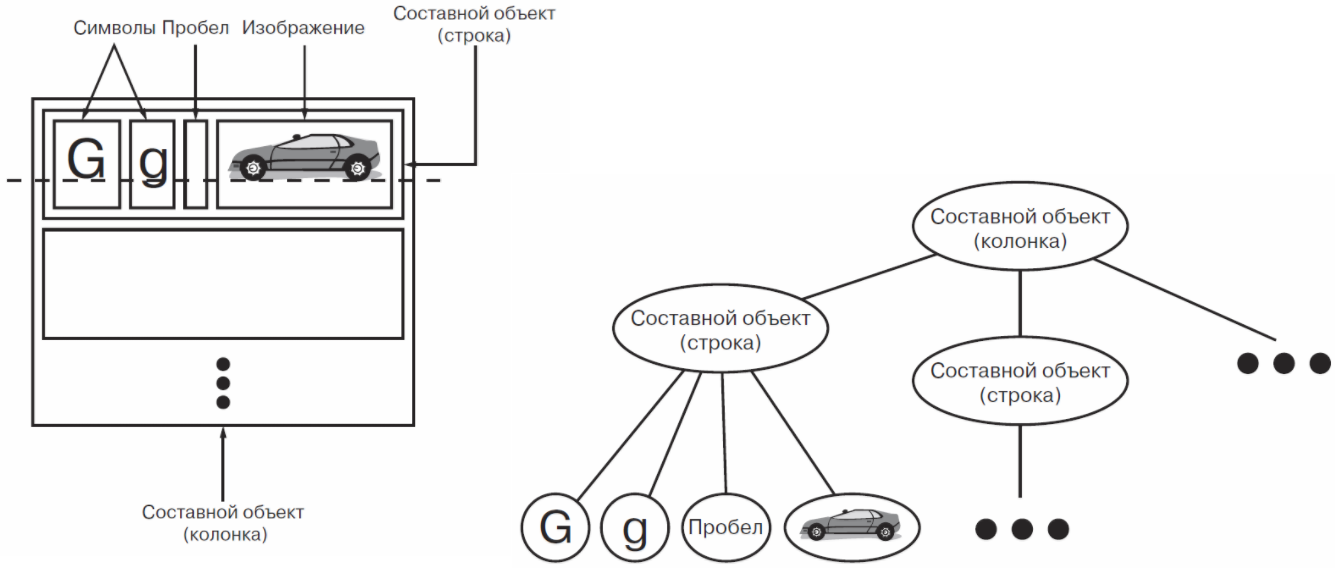
\includegraphics[width=0.9\textwidth]{recursiveComposition.png}
            \attribution{Э. Гамма и др., Приемы объектно-ориентированного проектирования}
        \end{center}
    \end{frame}

    \begin{frame}
        \frametitle{Диаграмма классов: глифы}
        \begin{center}
            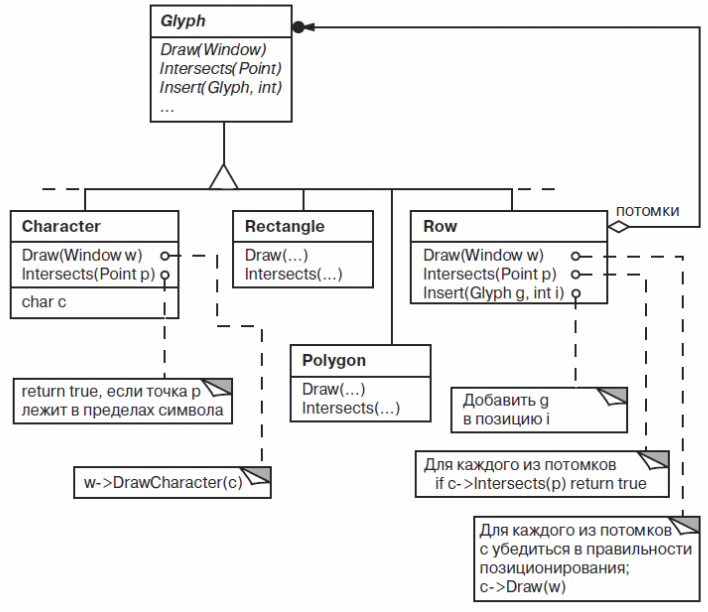
\includegraphics[width=0.6\textwidth]{glyphs.png}
            \attribution{Э. Гамма и др., Приемы объектно-ориентированного проектирования}
        \end{center}
    \end{frame}

    \begin{frame}
        \frametitle{Паттерн ``Компоновщик''}
        \framesubtitle{Composite}
        \begin{columns}
            \begin{column}{0.5\textwidth}
                \begin{itemize}
                    \item Представление иерархии объектов вида часть-целое
                    \item Единообразная обработка простых и составных объектов
                    \item Простота добавления новых компонентов
                    \item Пример:
                    \begin{itemize}
                        \item Синтаксические деревья
                    \end{itemize}
                \end{itemize}
            \end{column}
            \begin{column}{0.5\textwidth}
                \begin{center}
                    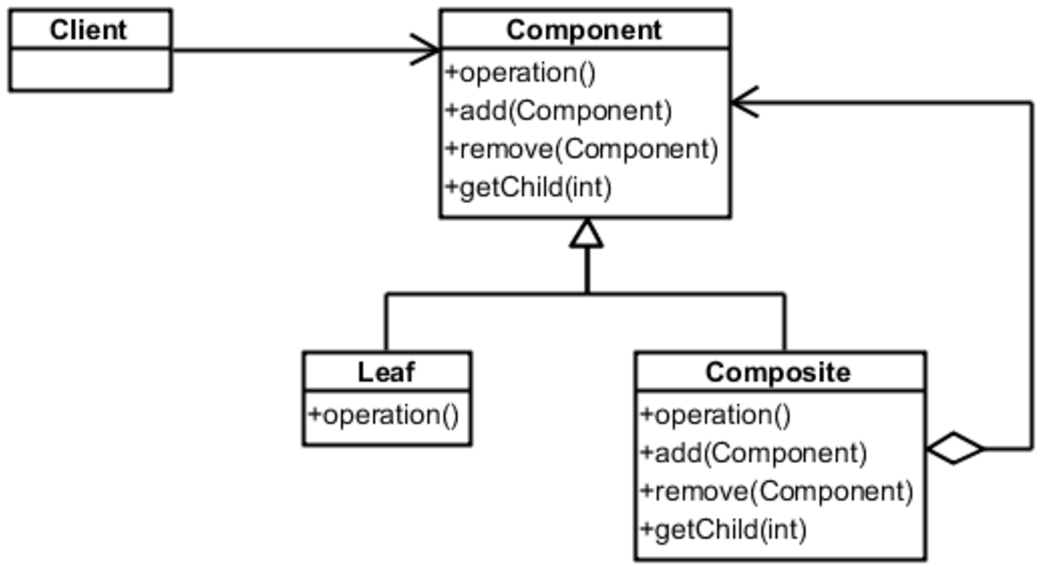
\includegraphics[width=\textwidth]{composite.png}
                \end{center}
            \end{column}
        \end{columns}
    \end{frame}

    \begin{frame}
        \frametitle{``Компоновщик'' (Composite), детали реализации}
        \begin{itemize}
            \item Идеологические проблемы с операциями для работы с потомками
            \begin{itemize}
                \item Не имеют смысла для листа
                \begin{itemize}
                    \item Можно считать Leaf Composite-ом, у которого всегда 0 потомков
                \end{itemize}
                \item Операции add и remove можно объявить и в Composite, тогда придётся делать cast
                \begin{itemize}
                    \item Иначе надо бросать исключения в add и remove
                \end{itemize}
            \end{itemize}
            \item Операция getComposite() –-- более аккуратный аналог cast-а
            \item Где определять список потомков
            \begin{itemize}
                \item В Composite, экономия памяти
                \item В Component, единообразие операций
                \item ``Список'' вполне может быть хеш-таблицей, деревом или чем угодно
            \end{itemize}
        \end{itemize}
    \end{frame}

    \begin{frame}
        \frametitle{``Компоновщик'', детали реализации (2)}
        \begin{itemize}
            \item Ссылка на родителя
            \begin{itemize}
                \item Может быть полезна для простоты обхода
                \item ``Цепочка обязанностей''
                \item Но дополнительный инвариант
                \item Обычно реализуется в Component
            \end{itemize}
            \item Разделяемые поддеревья и листья
            \begin{itemize}
                \item Позволяют сильно экономить память
                \item Проблемы с навигацией к родителям и разделяемым состоянием
                \item Паттерн ``Приспособленец''
            \end{itemize}
            \item Порядок потомков может быть важен, может нет
            \item Кеширование информации для обхода или поиска
            \begin{itemize}
                \item Например, кеширование ограничивающих прямоугольников для фрагментов картинки
                \item Инвалидация кеша
            \end{itemize}
            \item Удаление потомков
            \begin{itemize}
                \item Если нет сборки мусора, то лучше в Composite
                \item Следует опасаться разделяемых листьев/поддеревьев
            \end{itemize}
        \end{itemize}
    \end{frame}

    \section{Паттерн ``Декоратор''}

    \begin{frame}
        \frametitle{Усовершенствование UI}
        \begin{itemize}
            \item Хотим сделать рамку вокруг текста и полосы прокрутки, отключаемые по опции
            \item Желательно убирать и добавлять элементы обрамления так, чтобы другие объекты даже не знали, что они есть
            \item Хотим менять во время выполнения --- наследование не подойдёт
            \begin{itemize}
                \item Наш выбор ­--- композиция
                \item Прозрачное обрамление
            \end{itemize}
        \end{itemize}
    \end{frame}

    \begin{frame}
        \frametitle{Моноглиф}
        \begin{columns}
            \begin{column}{0.6\textwidth}
                \begin{itemize}
                    \item Абстрактный класс с ровно одним сыном
                    \begin{itemize}
                        \item Вырожденный случай компоновщика
                    \end{itemize}
                    \item ``Обрамляет'' сына, добавляя новую функциональность
                \end{itemize}
            \end{column}
            \begin{column}{0.4\textwidth}
                \begin{center}
                    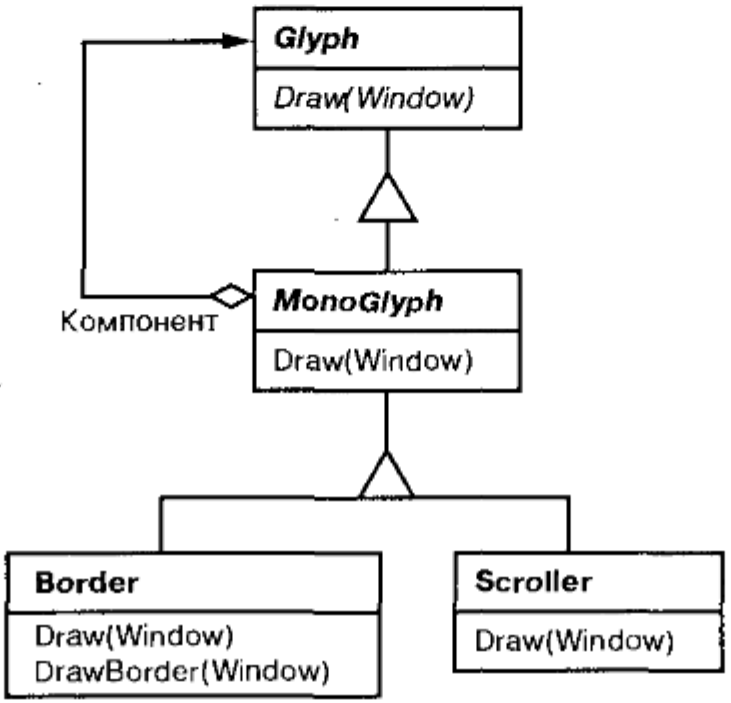
\includegraphics[width=0.9\textwidth]{monoglyph.png}
                    \attribution{Э. Гамма и др., Приемы объектно-ориентированного проектирования}
                \end{center}
            \end{column}
        \end{columns}
    \end{frame}

    \begin{frame}
        \frametitle{Структура глифов}
        \begin{center}
            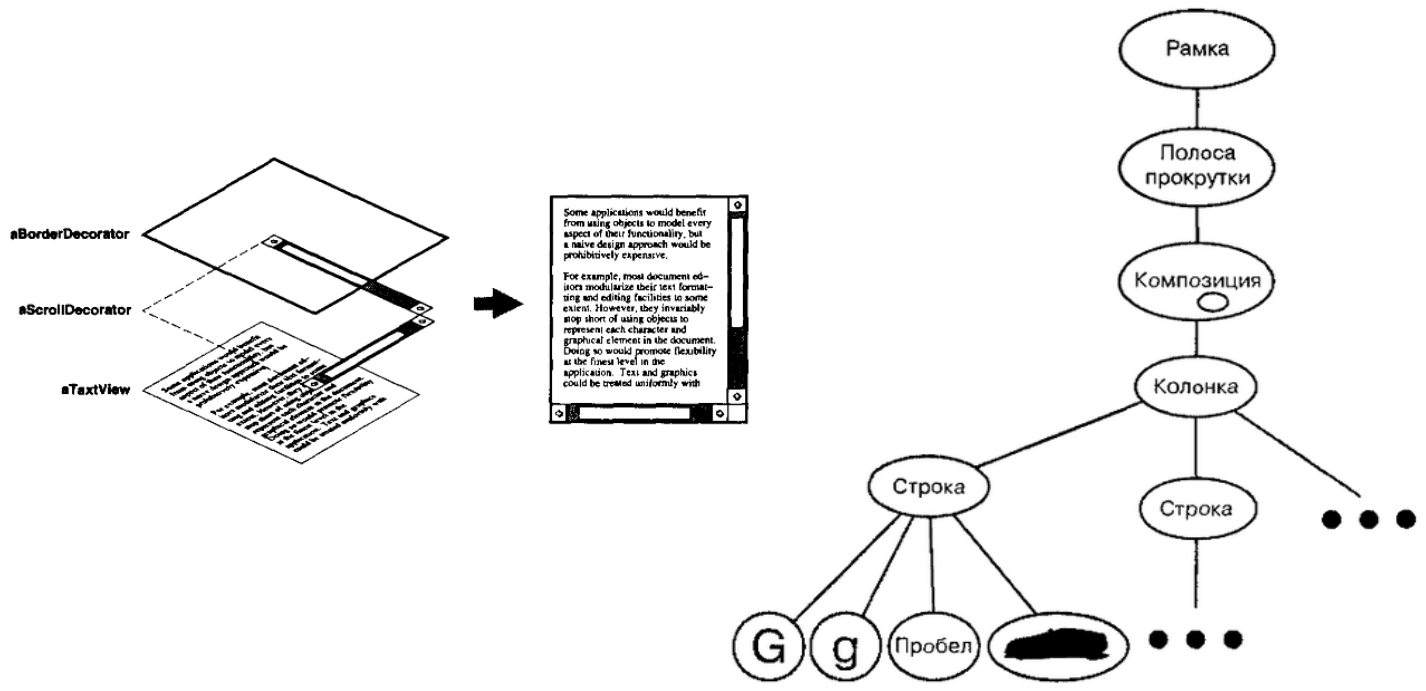
\includegraphics[width=0.9\textwidth]{glyphStructure.png}
            \attribution{Э. Гамма и др., Приемы объектно-ориентированного проектирования}
        \end{center}
    \end{frame}

    \begin{frame}
        \frametitle{Паттерн ``Декоратор''}
        \framesubtitle{Decorator}
        \begin{center}
            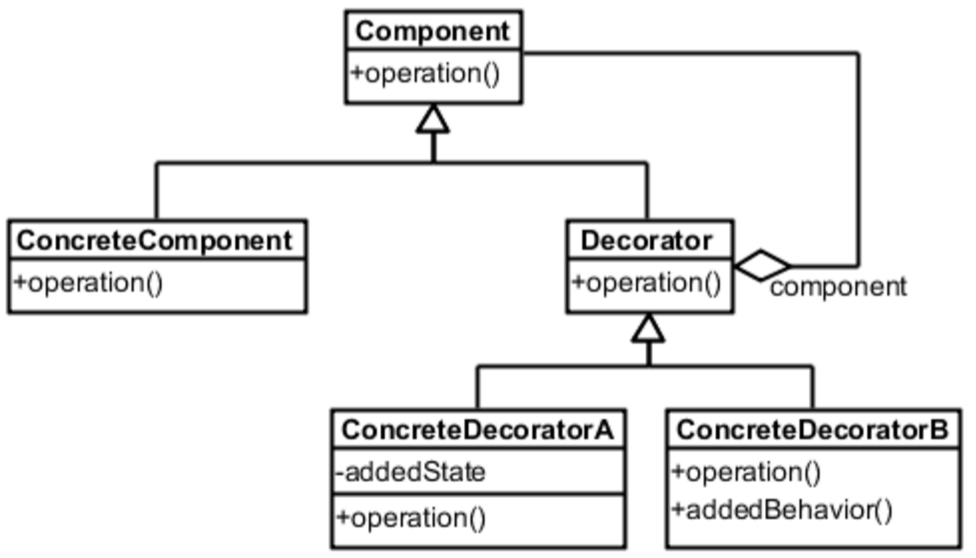
\includegraphics[width=0.6\textwidth]{decorator.png}
        \end{center}
    \end{frame}

    \begin{frame}
        \frametitle{Декоратор, особенности}
        \begin{itemize}
            \item Динамическое добавление (и удаление) обязанностей объектов
            \begin{itemize}
                \item Большая гибкость, чем у наследования
            \end{itemize}
            \item Позволяет избежать перегруженных функциональностью базовых классов
            \item Много мелких объектов
        \end{itemize}
    \end{frame}

    \begin{frame}
        \frametitle{``Декоратор'' (Decorator), детали реализации}
        \begin{columns}
            \begin{column}{0.6\textwidth}
                \begin{itemize}
                    \item Интерфейс декоратора должен соответствовать интерфейсу декорируемого объекта
                    \begin{itemize}
                        \item Иначе получится ``Адаптер''
                    \end{itemize}
                    \item Если конкретный декоратор один, абстрактный класс можно не делать
                \end{itemize}
            \end{column}
            \begin{column}{0.4\textwidth}
                \begin{center}
                    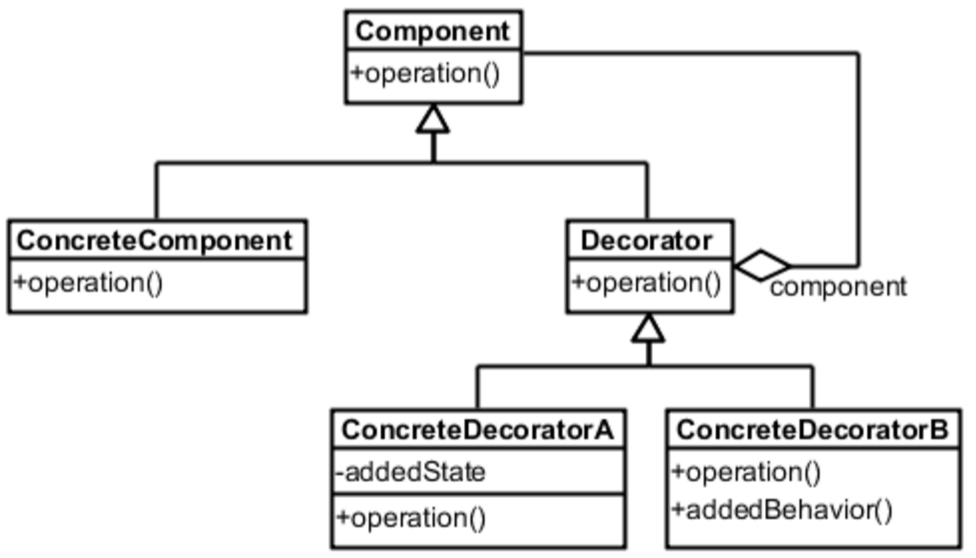
\includegraphics[width=\textwidth]{decorator.png}
                \end{center}
            \end{column}
        \end{columns}
        \begin{itemize}
            \item Component должен быть по возможности небольшим (в идеале, интерфейсом)
            \begin{itemize}
                \item Иначе лучше паттерн ``Стратегия''
                \item Или самодельный аналог, например, список ``расширений'', которые вызываются декорируемым объектом вручную перед операцией или после неё
            \end{itemize}
        \end{itemize}
    \end{frame}

    \section{Паттерн ``Стратегия''}

    \begin{frame}
        \frametitle{Форматирование текста}
        \begin{itemize}
            \item Задача --- разбиение текста на строки, колонки и т.д.
            \item Высокоуровневые параметры форматирования
            \begin{itemize}
                \item Ширина полей, размер отступа, межстрочный интервал и т.д.
            \end{itemize}
            \item Компромисс между качеством и скоростью работы
            \item Инкапсуляция алгоритма
        \end{itemize}
    \end{frame}

    \begin{frame}
        \frametitle{Compositor и Composition}
        \begin{center}
            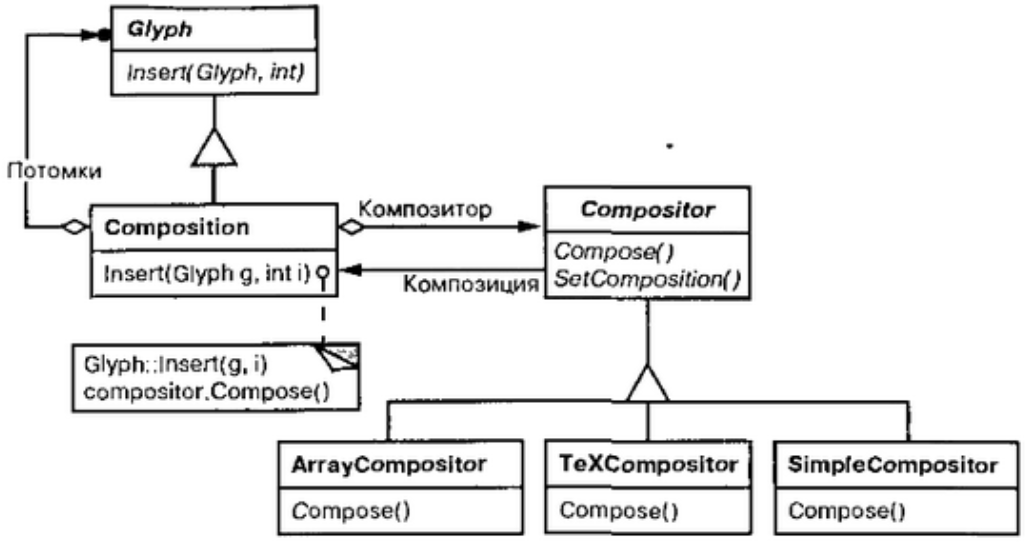
\includegraphics[width=0.7\textwidth]{compositor.png}
            \attribution{Э. Гамма и др., Приемы объектно-ориентированного проектирования}
        \end{center}
    \end{frame}

    \begin{frame}
        \frametitle{Паттерн ``Стратегия''}
        \framesubtitle{Strategy}
        \begin{itemize}
            \item Назначение --- инкапсуляция алгоритма в объект
            \item Самое важное --- спроектировать интерфейсы стратегии и контекста
            \begin{itemize}
                \item Так, чтобы не менять их для каждой стратегии
            \end{itemize}
            \item Применяется, если
            \begin{itemize}
                \item Имеется много родственных классов с разным поведением
                \item Нужно иметь несколько вариантов алгоритма
                \item В алгоритме есть данные, про которые клиенту знать не надо
                \item В коде много условных операторов
            \end{itemize}
        \end{itemize}
        \begin{center}
            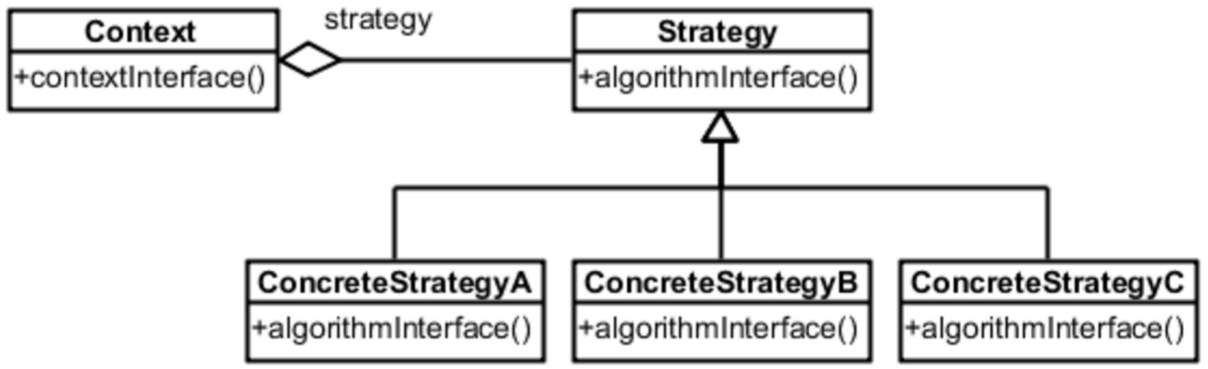
\includegraphics[width=0.6\textwidth]{strategy.png}
        \end{center}
    \end{frame}

    \begin{frame}
        \frametitle{``Стратегия'' (Strategy), детали реализации}
        \begin{center}
            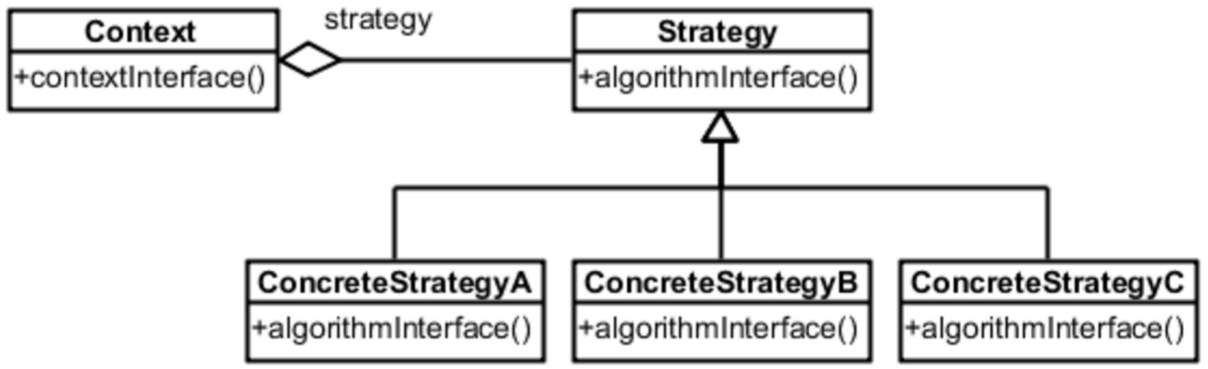
\includegraphics[width=0.6\textwidth]{strategy.png}
        \end{center}
        \begin{itemize}
            \item Передача контекста вычислений в стратегию
            \begin{itemize}
                \item Как параметры метода --- уменьшает связность, но некоторые параметры могут быть стратегии не нужны
                \item Передавать сам контекст в качестве аргумента --- в Context интерфейс для доступа к данным
            \end{itemize}
        \end{itemize}
    \end{frame}

    \begin{frame}
        \frametitle{``Стратегия'' (Strategy), детали реализации (2)}
        \begin{itemize}
            \item Стратегия может быть параметром шаблона
            \begin{itemize}
                \item Если не надо её менять на лету
                \item Не надо абстрактного класса и нет оверхеда на вызов виртуальных методов
            \end{itemize}
            \item Стратегия по умолчанию
            \begin{itemize}
                \item Или просто поведение по умолчанию, если стратегия не установлена
            \end{itemize}
            \item Объект-стратегия может быть приспособленцем
        \end{itemize}
    \end{frame}

    \section{Паттерн ``Адаптер''}

    \begin{frame}
        \frametitle{Проблема неподходящих интерфейсов}
        \begin{itemize}
            \item Графический редактор
            \begin{itemize}
                \item Shape, Line, Polygon, ...
            \end{itemize}
            \item Сторонний класс TextView
            \begin{itemize}
                \item Хотим его реализацию
                \item Другой интерфейс
            \end{itemize}
        \end{itemize}
        \vspace{2mm}
        \begin{center}
            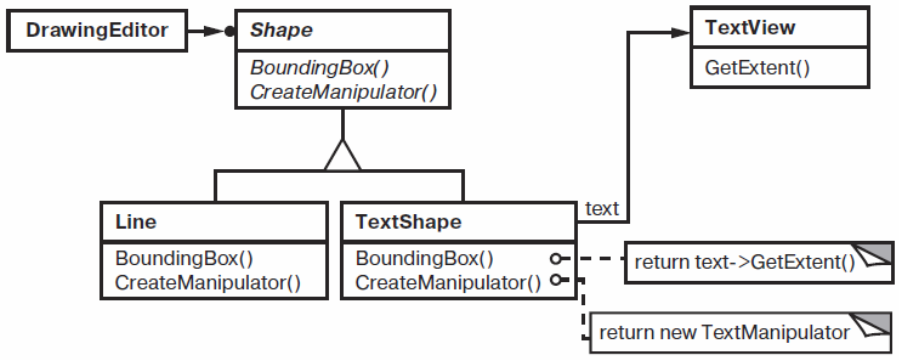
\includegraphics[width=0.6\textwidth]{adapterExample.png}
            \attribution{Э. Гамма и др., Приемы объектно-ориентированного проектирования}
        \end{center}
    \end{frame}

    \begin{frame}
        \frametitle{Паттерн ``Адаптер''}
        \framesubtitle{Adapter}
        \begin{columns}
            \begin{column}{0.5\textwidth}
                \begin{itemize}
                    \item Адаптер объекта:
                        \vspace{0.3cm}
                        
                        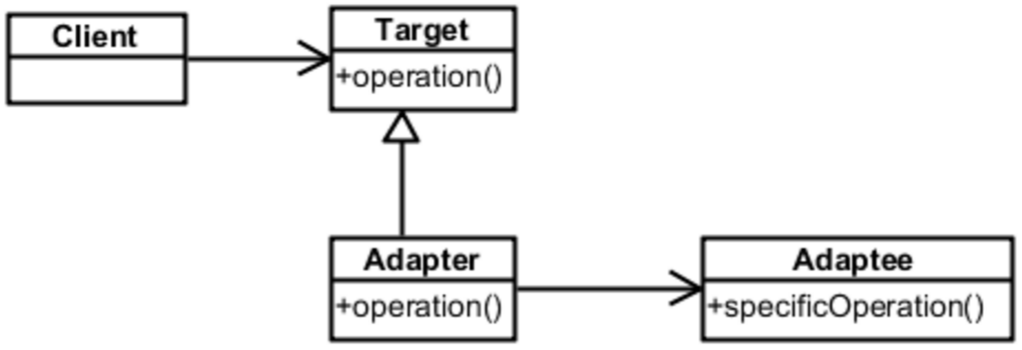
\includegraphics[width=0.8\textwidth]{objectAdapter.png}
                \end{itemize}
            \end{column}
            \begin{column}{0.5\textwidth}
                \begin{itemize}
                    \item Адаптер класса:
                        \vspace{0.3cm}
                        
                        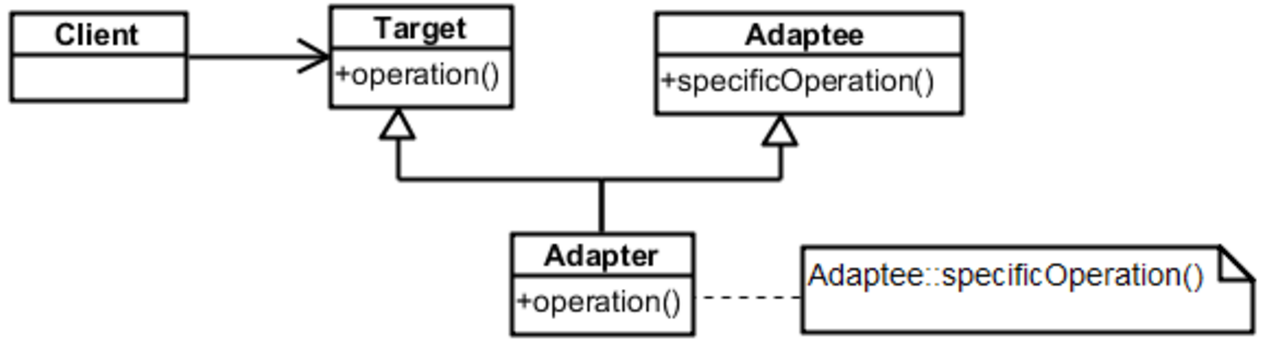
\includegraphics[width=0.9\textwidth]{classAdapter.png}
                        \vspace{0.3cm}
                    \item private-наследование в C++
                \end{itemize}
            \end{column}
        \end{columns}
    \end{frame}

    \section{Паттерн ``Заместитель''}

    \begin{frame}
        \frametitle{Управление доступом к объектам}
        \begin{itemize}
            \item Встраивание в документ графических объектов
            \begin{itemize}
                \item Затраты на создание могут быть значительными
                \item Хотим отложить их на момент использования
            \end{itemize}
            \item Использование заместителей объектов
        \end{itemize}
        \vspace{3mm}
        \begin{center}
            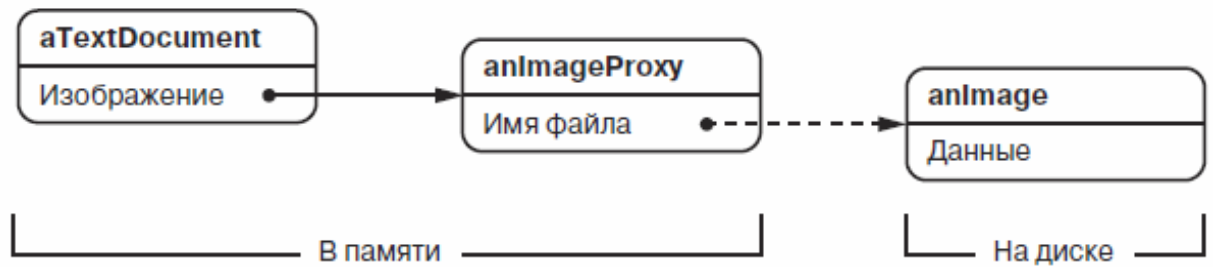
\includegraphics[width=0.6\textwidth]{proxyExample.png}
        \end{center}
    \end{frame}

    \begin{frame}
        \frametitle{Отложенная загрузка изображения}
        \begin{center}
            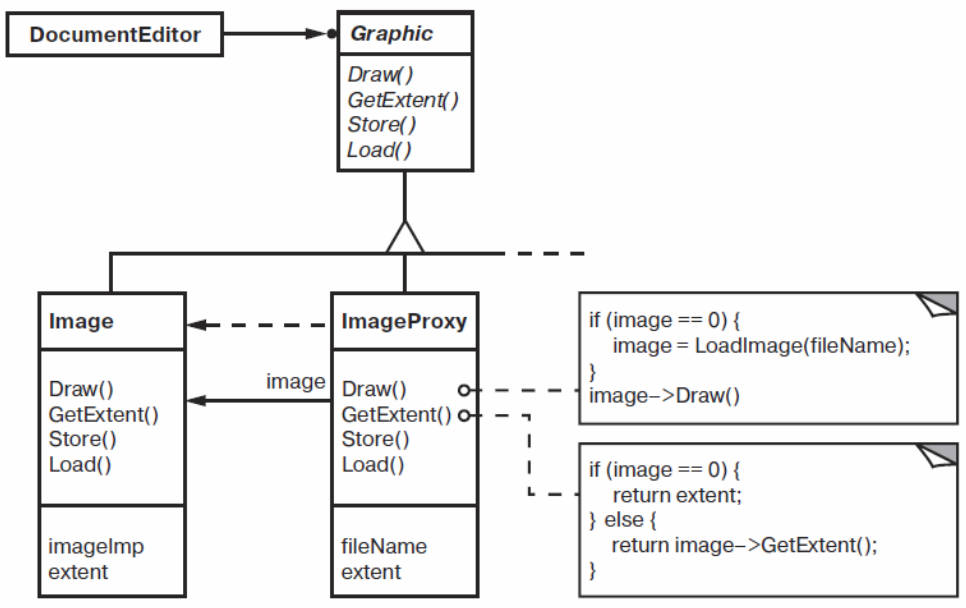
\includegraphics[width=0.7\textwidth]{proxyExampleClassDiagram.png}
        \end{center}
    \end{frame}

    \begin{frame}
        \frametitle{Паттерн ``Заместитель''}
        \framesubtitle{Proxy}
        \begin{center}
            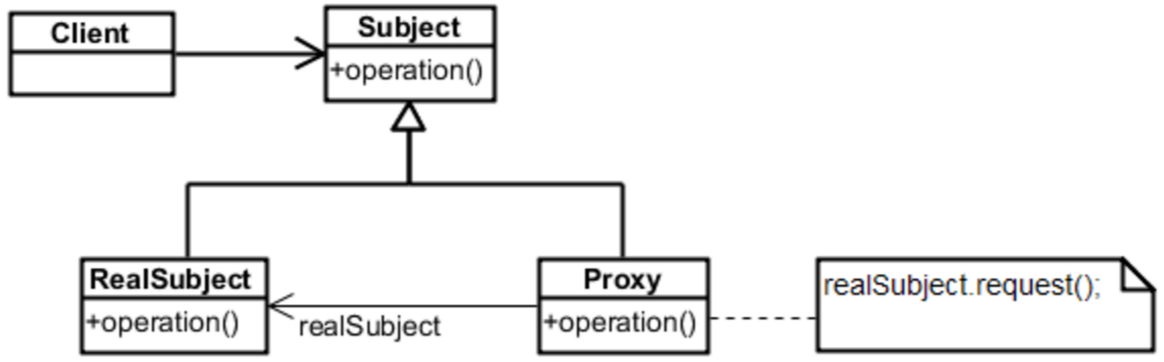
\includegraphics[width=0.6\textwidth]{proxy.png}
        \end{center}
        \begin{itemize}
            \item Замещение удалённых объектов
            \item Создание ``тяжёлых'' объектов по требованию
            \item Контроль доступа
            \item Умные указатели
            \begin{itemize}
                \item Подсчёт ссылок
                \item Ленивая загрузка/инициализация
                \item Работа с блокировками
                \item Копирование при записи
            \end{itemize}
        \end{itemize}
    \end{frame}

    \begin{frame}
        \frametitle{``Заместитель'', детали реализации}
        \begin{center}
            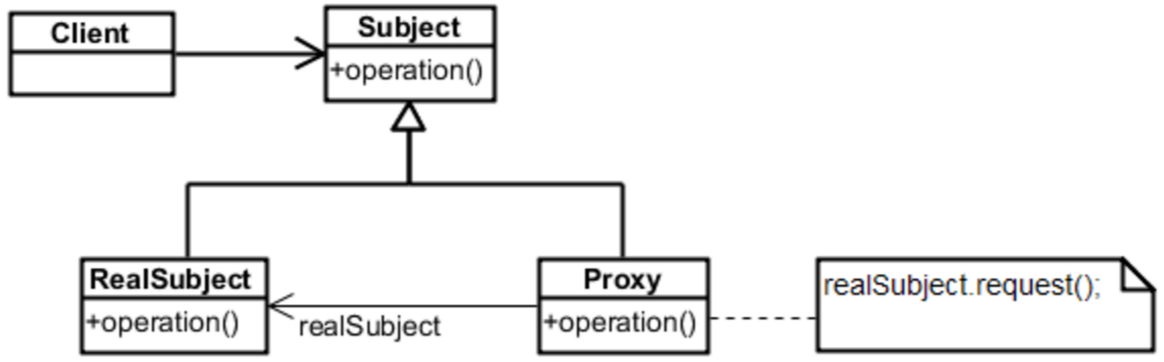
\includegraphics[width=0.6\textwidth]{proxy.png}
        \end{center}
        \begin{itemize}
            \item Перегрузка оператора доступа к членам класса (для C++)
            \begin{itemize}
                \item Умные указатели так устроены
                \item C++ вызывает операторы \mintinline{c++}|->| по цепочке
                \begin{itemize}
                    \item \mintinline{c++}|object->do()| может быть хоть \mintinline{c++}|((object.operator->()).operator->()).do()|
                \end{itemize}
                \item Не подходит, если надо различать операции
            \end{itemize}
        \end{itemize}
    \end{frame}

    \begin{frame}
        \frametitle{``Заместитель'', детали реализации (2)}
        \begin{itemize}
            \item Реализация ``вручную'' всех методов проксируемого объекта
            \begin{itemize}
                \item Сотня методов по одной строчке каждый
                \item C\#/F\#: \mintinline{csharp}|public void do() => realSubject.do();|
                \item Препроцессор/генерация
                \begin{itemize}
                    \item Технологии наподобие WCF
                \end{itemize}
            \end{itemize}
            \item Проксируемого объекта может не быть в памяти
        \end{itemize}
    \end{frame}

    \section{Паттерн ``Фасад''}

    \begin{frame}
        \frametitle{Паттерн ``Фасад''}
        \framesubtitle{Facade}
        \begin{columns}
            \begin{column}{0.4\textwidth}
                \begin{itemize}
                    \item Простой интерфейс к сложной системе
                    \item Отделение подсистем от клиента и друг от друга
                    \item Многоуровневая архитектура
                \end{itemize}
            \end{column}
            \begin{column}{0.6\textwidth}
                \begin{center}
                    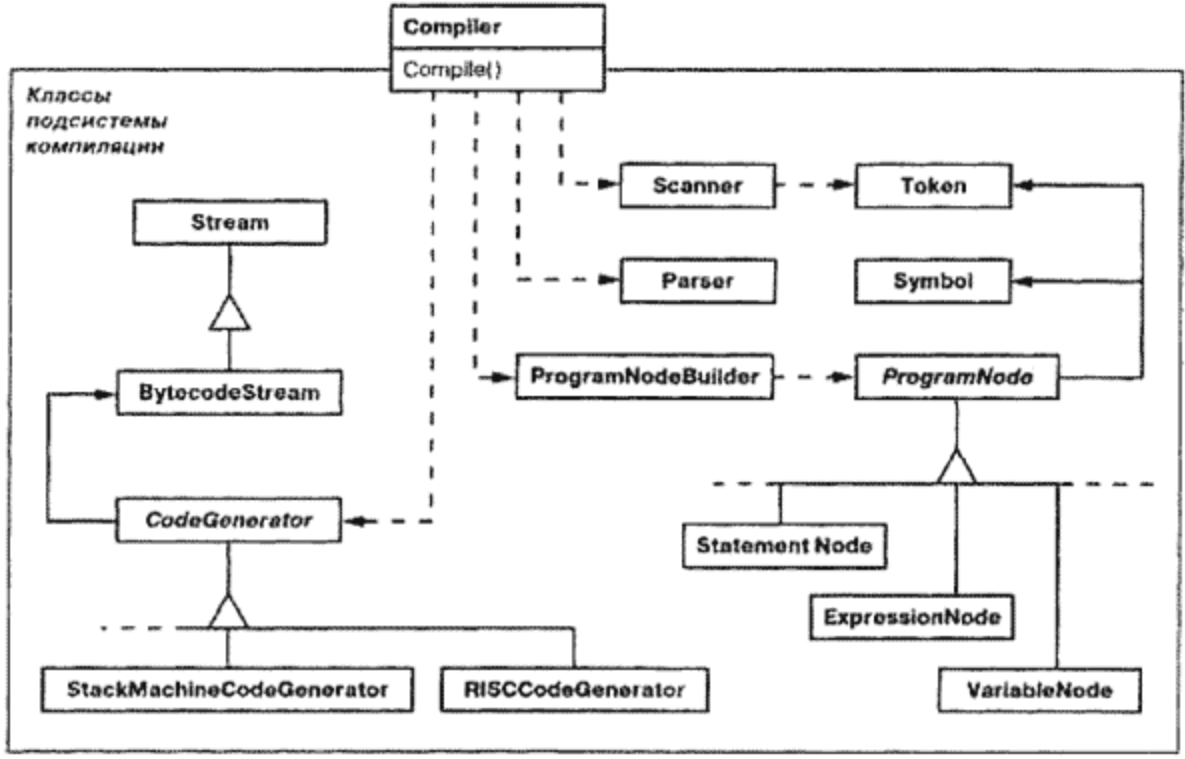
\includegraphics[width=0.9\textwidth]{facadeMotivation.png}
                    \attribution{Э. Гамма и др., Приемы объектно-ориентированного проектирования}
                \end{center}
            \end{column}
        \end{columns}
    \end{frame}

    \begin{frame}
        \frametitle{``Фасад'' (Facade), детали реализации}
        \begin{columns}
            \begin{column}{0.5\textwidth}
                \begin{itemize}
                    \item Абстрактный Facade
                    \begin{itemize}
                        \item Существенно снижает связность клиента с подсистемой
                    \end{itemize}
                \end{itemize}
            \end{column}
            \begin{column}{0.5\textwidth}
                \begin{center}
                    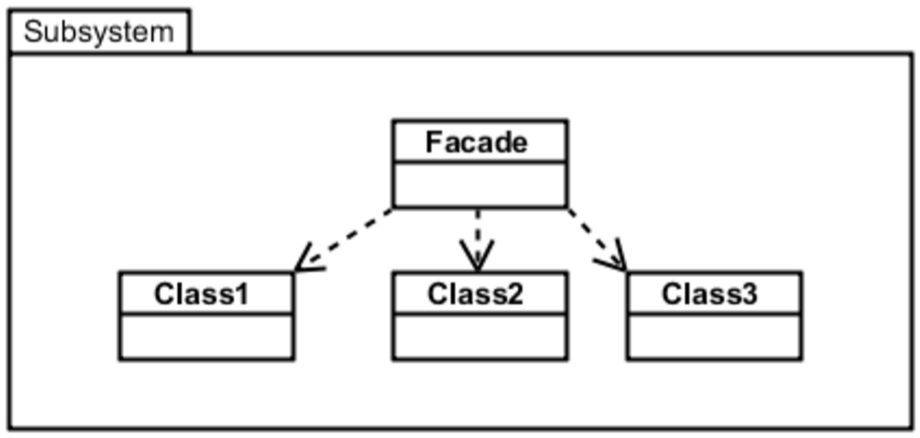
\includegraphics[width=0.8\textwidth]{facade.png}
                \end{center}
            \end{column}
        \end{columns}
        \begin{itemize}
            \item Открытые и закрытые классы подсистемы
            \begin{itemize}
                \item Пространства имён и пакеты помогают, но требуют дополнительных соглашений
                \begin{itemize}
                    \item Пространство имён details
                \end{itemize}
                \item Инкапсуляция целой подсистемы --- это хорошо
            \end{itemize}
        \end{itemize}
    \end{frame}

    \section{Паттерн ``Приспособленец''}

    \begin{frame}
        \frametitle{Паттерн ``Приспособленец'' (Flyweight)}
        Предназначается для эффективной поддержки множества мелких объектов

        Пример:

        \begin{itemize}
            \item Есть текстовый редактор
            \item Хочется работать с каждым символом как с объектом
            \begin{itemize}
                \item Единообразие алгоритмов форматирования и внутренней структуры документа
                \item Более красивая и ООПшная реализация
                \begin{itemize}
                    \item Паттерн ``Компоновщик'', структура ``Символ'' $\rightarrow$ ``Строка'' $\rightarrow$ ``Страница''
                \end{itemize}
            \end{itemize}
            \item Наивная реализация привела бы к чрезмерной расточительности по времени работы и по памяти, потому что документы с миллионами символов не редкость
        \end{itemize}
    \end{frame}

    \begin{frame}
        \frametitle{``Приспособленец'', пример}
        \begin{center}
            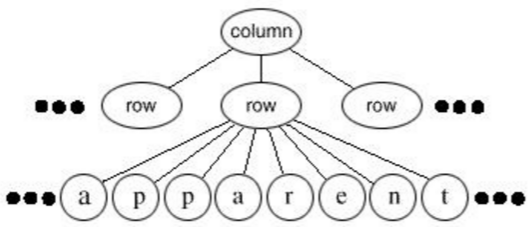
\includegraphics[width=0.38\textwidth]{noFlyweight.png}
            \raisebox{0.1\textheight}{\quad\Huge{$\rightarrow$}\quad}
            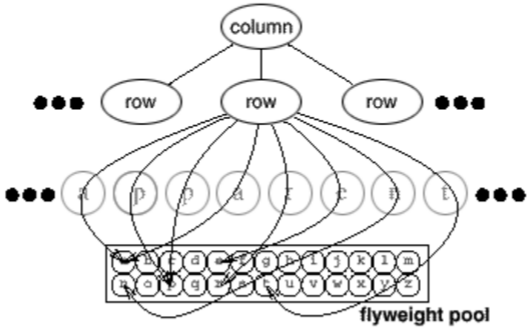
\includegraphics[width=0.38\textwidth]{flyweightExample.png}
        \end{center}
    \end{frame}

    \begin{frame}
        \frametitle{``Приспособленец'', общая схема}
        \begin{center}
            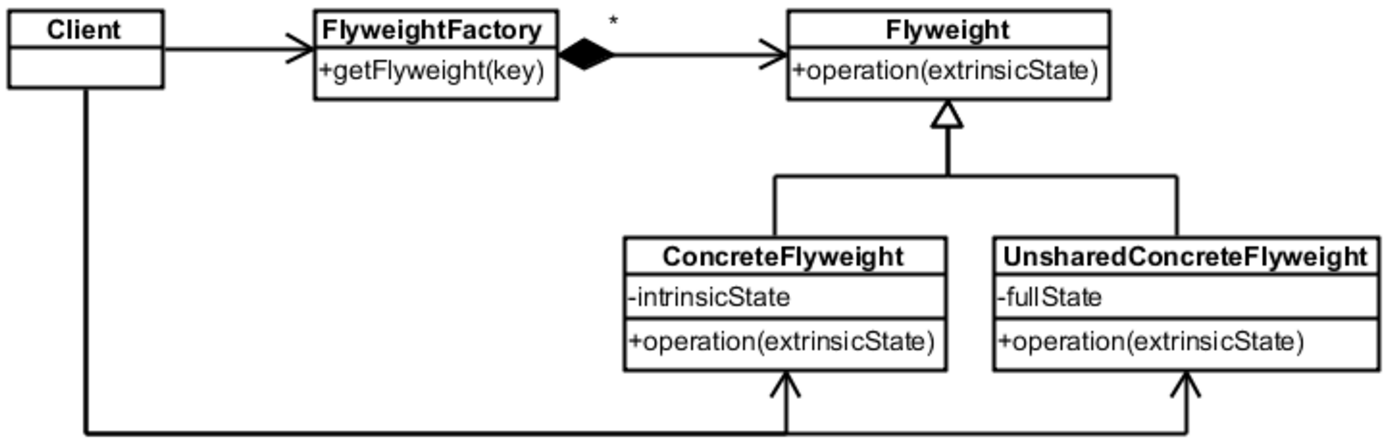
\includegraphics[width=0.7\textwidth]{flyweight.png}
        \end{center}
        \begin{footnotesize}
            \begin{itemize}
                \item \textit{Flyweight} --- определяет интерфейс, через который приспособленцы могут получать внешнее состояние
                \item \textit{ConcreteFlyweight} --- реализует интерфейс Flyweight и может иметь внутреннее состояние, не зависит от контекста
                \item \textit{UnsharedConcreteFlyweight} --- неразделяемый ``приспособленец'', хранящий всё состояние в себе, бывает нужен, чтобы собирать иерархические структуры из Flyweight-ов (``Компоновщик'')
                \item \textit{FlyweightFactory} --- содержит пул приспособленцев, создаёт их и управляет их жизнью
            \end{itemize}
        \end{footnotesize}
    \end{frame}

    \begin{frame}
        \frametitle{``Приспособленец'', диаграмма объектов}
        \begin{center}
            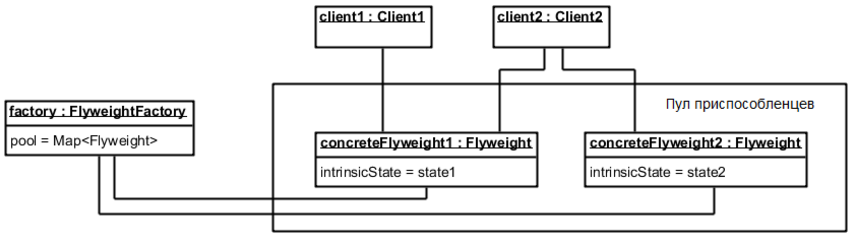
\includegraphics[width=0.8\textwidth]{flyweightObjects.png}
        \end{center}
        \begin{itemize}
            \item Клиенты могут быть разных типов
            \item Клиенты могут разделять приспособленцев
            \begin{itemize}
                \item Один клиент может иметь несколько ссылок на одного приспособленца
            \end{itemize}
            \item Во время выполнения клиенты имеют право не знать про фабрику
        \end{itemize}
    \end{frame}

    \begin{frame}
        \frametitle{Когда применять}
        \begin{itemize}
            \item Когда в приложении используется много мелких объектов
            \item Они допускают разделение состояния на внутреннее и внешнее
            \begin{itemize}
                \item Внешнее состояние было вычислимо
            \end{itemize}
            \item Идентичность объектов не важна
            \begin{itemize}
                \item Используется семантика Value Type
            \end{itemize}
            \item Главное, когда от такого разделения можно получить ощутимый выигрыш
        \end{itemize}
    \end{frame}

    \begin{frame}
        \frametitle{Тонкости реализации}
        \begin{itemize}
            \item Внешнее состояние --- по сути, отдельный объект, поэтому если различных внешних состояний столько же, сколько приспособленцев, смысла нет
            \begin{itemize}
                \item Один объект-состояние покрывает сразу несколько приспособленцев
                \begin{itemize}
                    \item Например, объект ``Range'' может хранить параметры форматирования для всех букв внутри фрагмента
                \end{itemize}
            \end{itemize}
            \item Клиенты не должны инстанцировать приспособленцев сами, иначе трудно обеспечить разделение
            \begin{itemize}
                \item Имеет смысл иметь механизм для удаления неиспользуемых приспособленцев
                \begin{itemize}
                    \item Если их может быть много
                \end{itemize}
            \end{itemize}
            \item Приспособленцы немутабельны и Value Objects (с правильно переопределённой операцией сравнения)
            \begin{itemize}
                \item Про hashCode() тоже надо не забыть
            \end{itemize}
        \end{itemize}
    \end{frame}

\end{document}
